\documentclass[14pt]{beamer}

\usepackage{graphicx}
\usepackage{listings}

\usepackage{helvet}

\usetheme{CambridgeUS}
\usecolortheme{seahorse}

\mode<presentation>

\title{Diving Into Flask}
\subtitle{Head On}

\author[A. Mishkovskyi]{Andrii V. Mishkovskyi \\ \texttt{contact@mishkovskyi.net}}
\date[EuroPython 2012]

\lstset{
  language=Python,
  % basicstyle=\ttfamily\scriptsize,
  basicstyle=\ttfamily\footnotesize,
  columns=fixed,
  showspaces=false,
  showstringspaces=false,
}

\AtBeginSection[]{
  \frame{\sectionpage}
}

\begin{document}

\frame{\titlepage}

\section{Warming up}

% Or should I do a "this guy" text + an arrow pointing to me?

% \begin{frame}{Who am I?}
%   \begin{itemize}
%   \item Developer for Hyves
%   \item Python fan
%   \item Heavy user of Flask (and Werkzeug in the past)
%   \end{itemize}
% \end{frame}

% \begin{frame}{What is Hyves?}
%   \begin{itemize}
%   \item The 2nd biggest social network in Netherlands
%   \item Used to be exclusively PHP shop
%   \item Primarily Python nowadays
%   \item And primarily Flask
%   \end{itemize}
% \end{frame}

\begin{frame}
  \frametitle{Presentation theme}
  \begin{itemize}
  \item Share our experience with Flask
  \item Explore inner workings of libraries we used
  \item Understand why things break
  \end{itemize}
\end{frame}

\begin{frame}
  \frametitle{Why Flask?}
  \only<1>{
    \begin{itemize}
    \item Well-documented
    \item Great API
    \item Easily extendable
    \item Well-suited for web APIs
    \end{itemize}
  }
  \only<2>{
    \begin{center}
      \LARGE{Yes, we also considered Django, Pyramid and many more}
    \end{center}
  }
\end{frame}

\section{Exploring Flask}

\subsection{Starting with the simplest}

\begin{frame}[fragile]
\only<1,2>{  \frametitle{Where we all start}}
\only<3>{\frametitle{Where some of us end up}}
  \only<1>{
    \lstinputlisting[language=Python]{code/simplest.py}
  }
  \only<2>{
    \lstinputlisting[language=Python,lastline=6,firstline=4]{code/simplest.py}
  }
  \only<3>{
    \lstinputlisting{code/complex-route.py}
  }
\end{frame}

\subsection{Flask views}

\begin{frame}
  \frametitle{Manual dispatch}
  \lstinputlisting{code/flask-routing-manual-dispatch.py}
\end{frame}

\begin{frame}
  \frametitle{Let Flask do all the hard work}
  \lstinputlisting{code/flask-routing-function-level.py}
\end{frame}

\begin{frame}
  \frametitle{Class views with manual dispatch}
  \lstinputlisting{code/flask-routing-class-based-manual-dispatch.py}
\end{frame}

\begin{frame}
  \frametitle{Class views with HTTP method-based dispatch}
  \lstinputlisting{code/flask-routing-class-based.py}
\end{frame}

\subsection{Simple, yet powerful}

\begin{frame}
  \frametitle{\texttt{Flask.route}}
  \begin{itemize}
  \item Decorator that calls \texttt{Flask.add\_url\_rule}
  \item \texttt{Flask.add\_url\_rule} creates \texttt{werkzeug.routing.Rule}
    and adds it to \texttt{werkzeug.routing.Map}
  \item \texttt{werkzeug.routing.Map} does the URL matching magic
  \end{itemize}
\end{frame}

\begin{frame}
  \frametitle{Class views}
\only<1>{
  \begin{itemize}
  \item Can't use Flask.route decorator
  \item Explicitly call \texttt{Flask.add\_url\_rule}
  \item \texttt{as\_view} method with creates the actual view function
  \end{itemize}
}
\only<2>{
  \lstinputlisting{code/flask-routing-class-based-views-as-view.py}
}

\end{frame}

\begin{frame}
  \frametitle{URL matching and decomposition}
  \only<1>{
    \begin{itemize}
    \item \texttt{Rule} creates regexp and collects proper converters
    \item \texttt{Map} holds all rules and builds the string for Rule to match
    \item \texttt{Converter}s convert the path parts into Python objects
    \end{itemize}
  }
  % Flask also tries to save some time matching URLs and sorts
  % Rules in specific order, see the key function for Rule
  \only<2>{\lstinputlisting{code/flask-routing-example.py}}
  \only<3>{\texttt{Rule} objects are stored in \texttt{Map} in sorted order.
    \lstinputlisting{code/flask-routing-rule-order.py}}
\end{frame}

\subsection{Blueprints}

\begin{frame}
  \frametitle{Modular Flask}
  \begin{itemize}
  \item More manageable
  \item No more interference with other's work
  \item Pluggable views
  \item Turnkey functionality implementations
  \end{itemize}
\end{frame}

\begin{frame}
  \frametitle{Introducing blueprints}
  \begin{itemize}
  \item We needed API versioning
  \item Instant win: \texttt{url\_prefix}
  \item Also splitting admin and API endpoints
  \item Ability to define per-blueprint template folder
  \end{itemize}
\end{frame}

\begin{frame}
  \frametitle{How blueprints work}
\only<1>{  \begin{itemize}
  \item Basically a proxy object
  \item That tracks if it was registered before
  \item The only interesting details is URL registration
  \end{itemize}
}
\only<2>{\lstinputlisting{code/flask-blueprints-example.py}}
\only<3>{\lstinputlisting{code/flask-blueprints-deferred-url-registration.py}}
\only<4>{\lstinputlisting{code/flask-blueprints-realize-url-registration.py}}
\end{frame}

\section{Flask and SQLAlchemy}

\subsection{Overview}

\begin{frame}
  \frametitle{Flask-SQLAlchemy}
\only<1>{
  \begin{itemize}
  \item Full of magic
  \item As in, dark magic
  \item Say, would you guess what is the purpose of this?
  \end{itemize}
}
\only<2>{
  \lstinputlisting{code/flask-sqlalchemy-riddle.py}
}
\only<3>{
  \begin{center}
  
\includegraphics[scale=0.6]{images/wtf-did-i-just-see.jpg}

  \end{center}
}
\end{frame}

\subsection{Partitioning}

\begin{frame}
  \frametitle{SQLAlchemy and binds}
\only<1>{
  \begin{itemize}
  \item Bind is the SQLAlchemy engine or pure connection object
  \item Flask-SQLAlchemy gives the ability to specify bind per model
  \item But sometimes one model has to reference several binds
  \end{itemize}
}
\only<2>{
  \lstinputlisting{code/flask-sqlalchemy-bind-example.py}
}
\end{frame}

\begin{frame}
  \frametitle{How Flask-SQLAlchemy does it}
  \lstinputlisting{code/flask-sqlalchemy-binds.py}
\end{frame}

\begin{frame}
  \frametitle{How do we achieve master-slave support?}
  \only<2>{
    \lstinputlisting[lastline=8]{code/flask-sqlalchemy-select-bind-explicitely.py}}
  \only<3>{
    \lstinputlisting[firstline=10]{code/flask-sqlalchemy-select-bind-explicitely.py}}
  % \only<2>{
  %   \lstinputlisting[firstline=10,lastline=17]{code/flask-sqlalchemy-select-bind-explicitely.py}}
  % \only<3>{
  %   \lstinputlisting[firstline=18]{code/flask-sqlalchemy-select-bind-explicitely.py}}
  \only<1>{
    \lstinputlisting{code/flask-sqlalchemy-bind-selection.py}
  }
\end{frame}

\subsection{Migrations}

\begin{frame}
  \frametitle{SQLAlchemy-migrate}
  \begin{itemize}
  \item Easy to start with
  \item Decent documentation
  \item Seems abandoned
  \item Had to write a wrapper to run \texttt{migrate} utility
  \end{itemize}
\end{frame}

\begin{frame}
  \frametitle{Alembic}
  \begin{itemize}
  \item 7 months ago seemed to be in alpha state
  \item Much more mature right now
  \item Great documentation, great implementation
  \item Written by Mike Bayer himself
  \end{itemize}
\end{frame}

\section{Deferring your tasks}

\subsection{Introducing celery}

\begin{frame}
  \frametitle{Celery features}
  \begin{itemize}
  \item Removes the hassle of using amqplib/pika
  \item Extensive set of features
  \item Confusing documentation
  \end{itemize}
\end{frame}

\begin{frame}
  \frametitle{Flask-Celery}
  \only<1>{
    \begin{itemize}
    \item Flask-Script is a requirement
    \item Most of the commands work
    \item Except for starting detached celery daemons
    \end{itemize}
  }
  \only<2>{\lstinputlisting{code/flask-celery-detached.py}}
\end{frame}


\subsection{Celery and logging}

\begin{frame}
\only<1,3>{
  \frametitle{Color formatting}
  \begin{block}{Problem}
    Celery always colorizes logs. We don't like colors.
  \end{block}
\only<3>{
  \begin{block}{Solution}
    Add \texttt{after\_setup\_logger} signal that reassigns all
    logging formatters for Celery logging handlers.
  \end{block}
}
}
\only<2>{
  \frametitle{OH HAI COLORZ}
  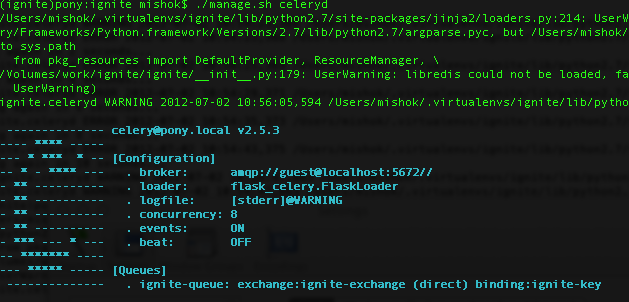
\includegraphics[scale=0.5]{images/celery-colored.png}
}
\end{frame}

% \begin{frame}
%   \frametitle{OH HEY COLORZ}
%   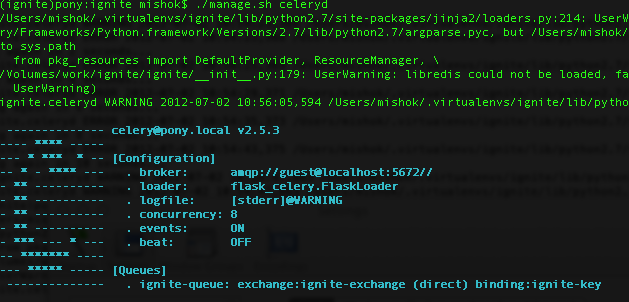
\includegraphics[scale=0.5]{images/celery-colored.png}
% \end{frame}

\begin{frame}
  \frametitle{Hijacking root logger}
  \begin{block}{Problem}
    Root logger is hijacked by Celery's logging setup, making your logging
    setup useless.
  \end{block}
  \begin{block}{Solution}
    Set \texttt{CELERYD\_HIJACK\_ROOT\_LOGGER} to \texttt{False}. Or better
    yet, never use root logger.
  \end{block}
\end{frame}

\begin{frame}
  \frametitle{Process name}
  \begin{block}{Problem}
    Logging might brake if you want to setup logging beyond log message
    format. \only<1>{
    See \texttt{https://gist.github.com/721870}
    \begin{quotation}
      There are three places in the code where the processName is written to a
      LogRecord, some of which can lead to unexpected behaviour in some scenarios
  \end{quotation}
}
  \end{block}
\only<2>{  \begin{block}{Solution}
    Avoid those scenarios.
  \end{block}
}
\end{frame}

\subsection{Monitoring Celery}

% https://github.com/celery/django-celery/blob/master/djcelery/snapshot.py

\begin{frame}
  \frametitle{Keeping an eye on Celery}
\only<1-2>{  \begin{itemize}
  \item Subclass \texttt{celery.events.snapshot.Polaroid}
    \only<1>{
    \item ???
    \item PROFIT
    }
    \only<2>{
    \item Implement \texttt{on\_shutter} method
    \item Check various metrics
    \item Generate report in whatever format you need
    }
  \end{itemize}
}
\only<3>{
  \lstinputlisting{code/celery-polaroid.py}
}
\end{frame}

\subsection{Celery and Flask-SQLAlchemy}

\begin{frame}
  \frametitle{Celery + SQLAlchemy + MySQL}
  \only<1>{
    \begin{block}{Problem}
      Each time worker starts, infamous \texttt{MySQL} error is raised:
      \begin{quotation}
        OperationalError:
        (2006, 'MySQL server has gone away')
      \end{quotation}
    \end{block}
    \begin{block}{Solution}
      Drop the whole connection (engine) pool at worker init.
    \end{block}
  }
  \only<2>{
    \lstinputlisting{code/celery-drop-sqlalchemy-connections.py}
  }
  \only<3>{
    \begin{block}{Problem}
      Session not closed if exception happens midway through transaction.
    \end{block}
    \begin{block}{Solution}
      Close the session in \texttt{task\_postrun} signal.
    \end{block}
  }
  \only<4>{
    \lstinputlisting{code/celery-close-session-unconditionally.py}
  }
  \only<5>{
    \begin{block}{Problem}
      Session still not closed properly if \alert{db object loses app context}.
      Worker hangs too if that happens.
      \begin{quotation}
        RuntimeError: application not registered on db instance
        and no application bound to current context
      \end{quotation}
    \end{block}
    \begin{block}{Solution}
      Close the session in \texttt{task\_postrun} signal \alert{but only
        if there was an exception}.
    \end{block}
  }
  \only<6>{
    \lstinputlisting{code/celery-close-session-unconditionally-proper.py}
  }
\end{frame}

\section{Caching \& profiling}

\subsection{Caching}

\begin{frame}
\only<1>{
  \frametitle{Flask-Cache}
  \begin{itemize}
  \item Plenty of caching decorators
  \item Otherwise -- thin wrapper around werkzeug.contrib.cache
  \end{itemize}
}
\only<2>{
  \frametitle{Really thin wrapper}
  \lstinputlisting{code/flask-cache-thin-wrapper.py}
}
\end{frame}

\begin{frame}
  \frametitle{Meh...}
  \begin{itemize}
  \item Wrote our own cache classes
  \item With namespace support
  \item And consistent hashing (based on libketama)
  \item Also fixed and improved Python libredis wrapper
  \end{itemize}
\end{frame}

\subsection{Profiling}

\begin{frame}
  \frametitle{statsd}
\only<1>{
  \begin{itemize}
  \item Use \texttt{python-statsd}
  \item I have no more bullet points to add here
  \item So, there
  \item ...
  \item A picture of a cat instead!
  \end{itemize}
}
\only<2>{
  \begin{center}
    
\includegraphics[scale=2.0]{images/bored-cat.jpg}
  \end{center}
}
\only<3>{\lstinputlisting{code/statsd-example.py}}
\end{frame}

\begin{frame}
  \frametitle{Flask-DebugToolbar}
  \begin{itemize}
  \item Direct port of Django's debug toolbar
  \item Great at identifying bottlenecks
  \item We also added memory profiling (Pympler)
  \item Also: great example for blueprint-based plugin
  \end{itemize}
\end{frame}

\section{Conclusion}

\begin{frame}
  \frametitle{Flask maturity}
  \begin{itemize}
  \item Flask is no longer an April Fool's joke
  \item Still micro, but not in terms of features
  \item You can and should build applications with Flask
  \item Flask is easy to reason about
  \end{itemize}
\end{frame}

\begin{frame}
  \frametitle{Flask's ecosystem}
  \begin{itemize}
  \item Not on par with Flask in places
  \item Interoperability is rough in places
  \item Lack's BDFL for extensions (mitsuhiko for president!)
  \end{itemize}
\end{frame}

\begin{frame}
  \begin{center}
    \LARGE{Questions?}
  \end{center}
\end{frame}

\end{document}
